% ta med damping på DP-delle

\documentclass[aspectratio=169,xcolor=dvipsnames]{beamer}
%\usetheme{SimplePlus}

\usepackage{hyperref}
\usepackage{graphicx} % Allows including images
\usepackage{booktabs} % Allows the use of \toprule, \midrule and \bottomrule in tables

%----------------------------------------------------------------------------------------
%	TITLE PAGE
%----------------------------------------------------------------------------------------

\title[PLS]{PLS IO koblinger} % The short title appears at the bottom of every slide, the full title is only on the title page
%\subtitle{Subtitle}

\author[Fred-Olav] {Fred-Olav Mosdal}

\institute[Fagskolen Rogaland VGS] % Your institution as it will appear on the bottom of every slide, may be shorthand to save space

\date{\today} % Date, can be changed to a custom date


%----------------------------------------------------------------------------------------
%	PRESENTATION SLIDES
%----------------------------------------------------------------------------------------

\begin{document}
\begin{frame}
\titlepage
	$$\includegraphics[width=4cm]{../../Fagskolen/StyringDel1/Fagskolen.jpg}$$
\end{frame}
\section{Digitale PLS inn- og utganger (IO-er)}


\begin{frame}
	\frametitle{Styringssystemers tre deler}
	\begin{columns}
		\begin{column}{0.5\textwidth}
	\begin{itemize}
		\item Inngangsenheter
		\item styreenheter 
		\item utgangsenheter
	\end{itemize}
		\end{column}
		\begin{column}{0.5\textwidth}
	$$\includegraphics[width=1\textwidth]{../output/noGPLimages/pls01.png}$$
		\end{column}
	\end{columns}
\end{frame}


\begin{frame}
	\frametitle{PLS-ens opprinnelse}
	\begin{columns}
		\begin{column}{0.5\textwidth}
			Ble lansert som erstatning for relestyringer\\
			Opprinnelsen sees fremdeles i det mest vanlige programeringsspråket for PLS-er Ladder Logic Diagram
		\end{column}
		\begin{column}{0.5\textwidth}
	$$\includegraphics[width=1\textwidth]{../output/noGPLimages/Modicon 084.jpg}$$
			\url{https://www.engineering.com/programmable-logic-controllers-the-evolution-of-a-disruptive-technology/}
		\end{column}
	\end{columns}
\end{frame}


\begin{frame}
	\frametitle{Eksempler på PLS-er}
$$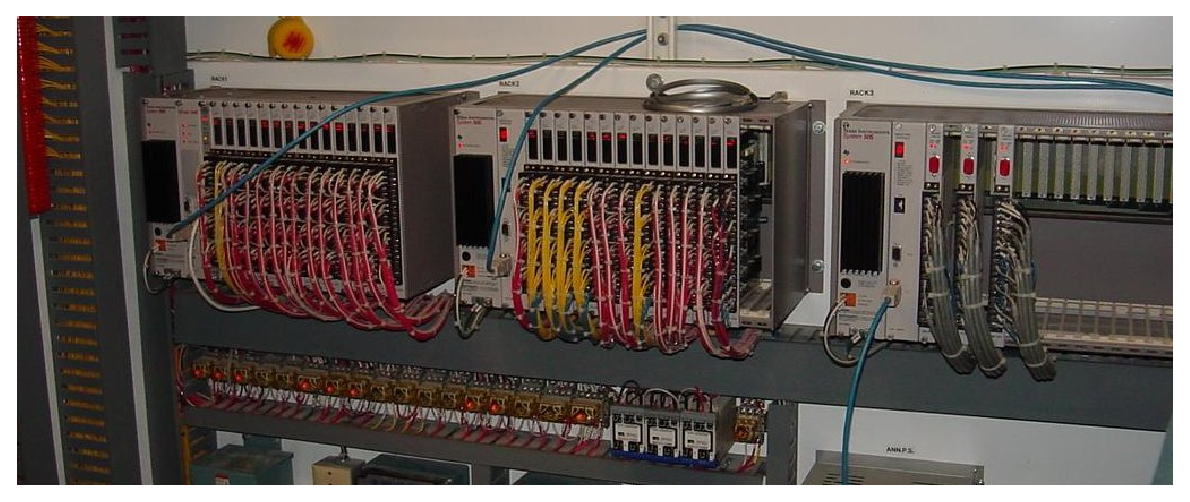
\includegraphics[width=1\textwidth]{plc_001.eps}$$
\end{frame}

\begin{frame}
	\frametitle{Eksempler på PLS-er}
$$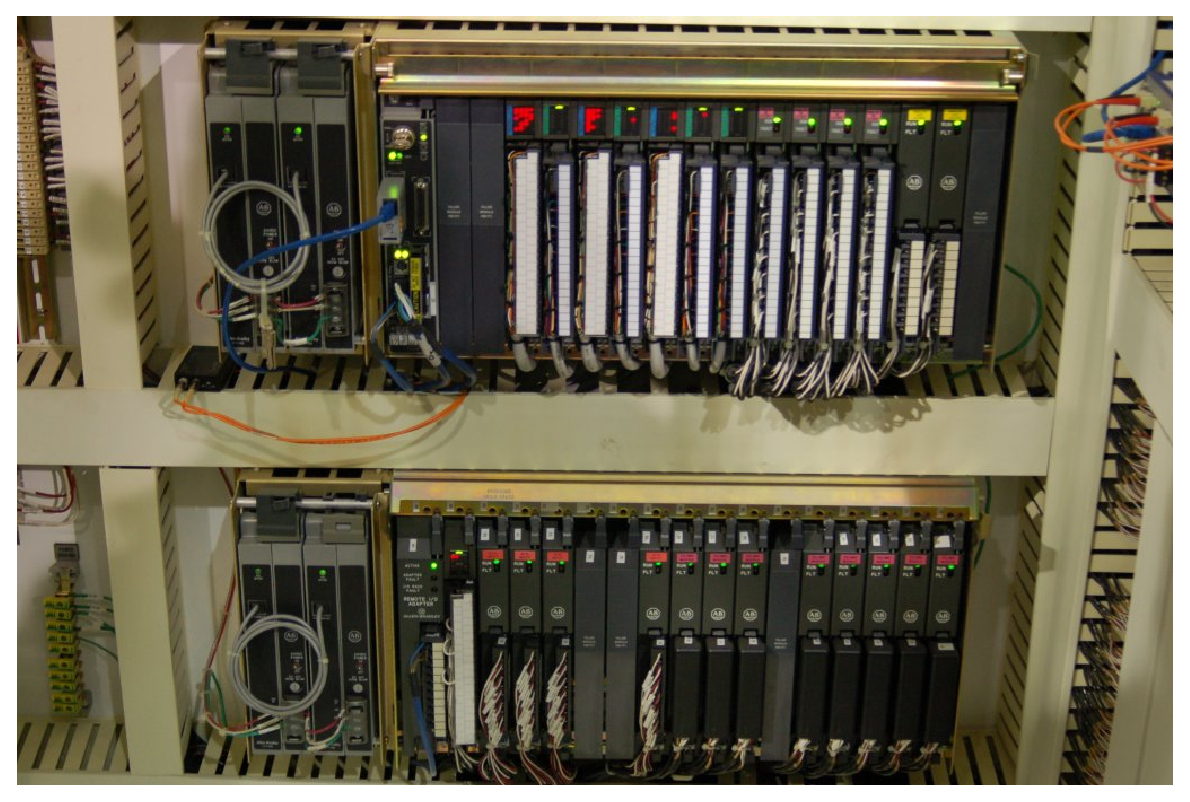
\includegraphics[width=0.8\textwidth]{plc_002.eps}$$
\end{frame}

\begin{frame}
	\frametitle{Eksempler på PLS-er}
$$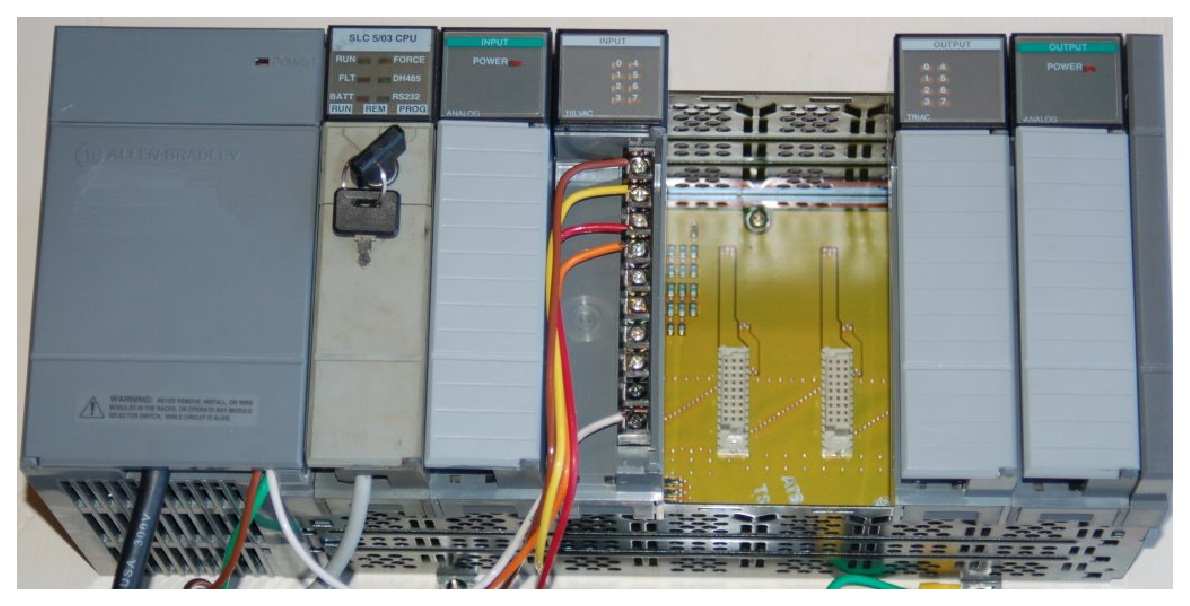
\includegraphics[width=0.9\textwidth]{plc_017.eps}$$
\end{frame}
\begin{frame}
	\frametitle{Eksempler på PLS-er}
$$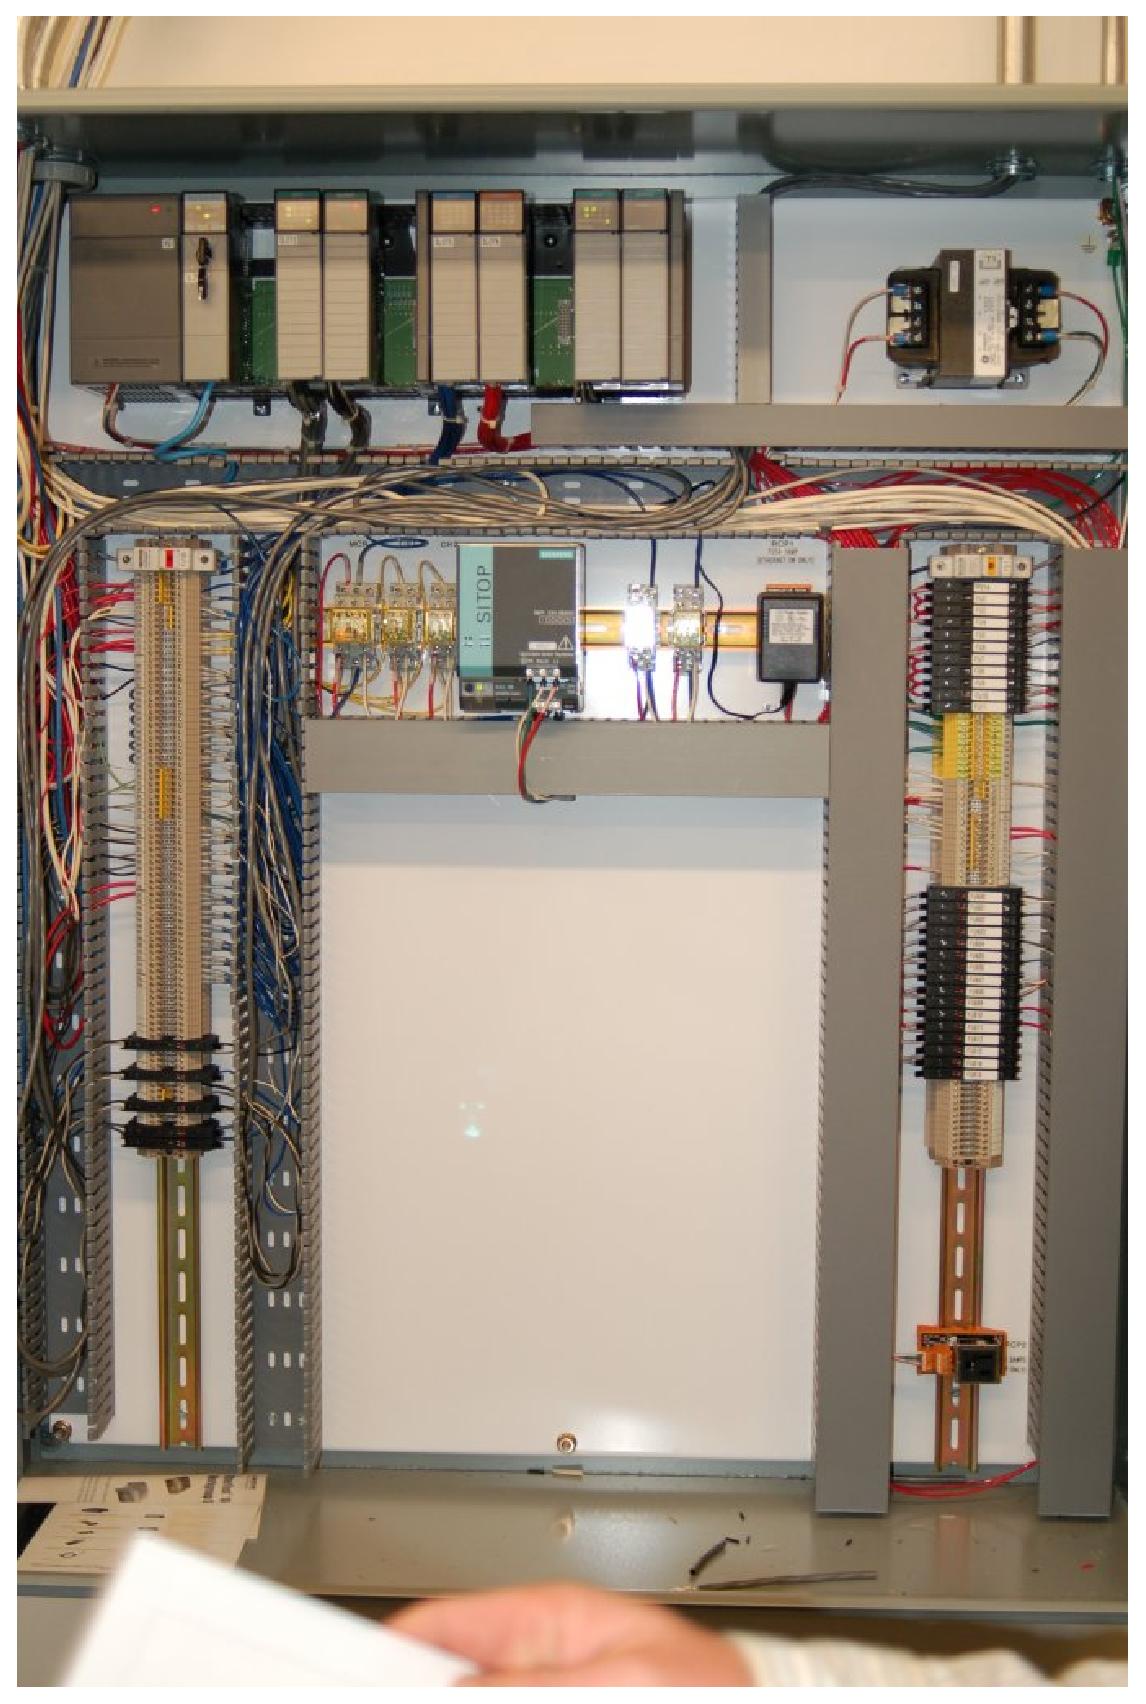
\includegraphics[width=0.8\textwidth]{plc_018.eps}$$
\end{frame}
\begin{frame}
	\frametitle{Eksempler på PLS-er}
$$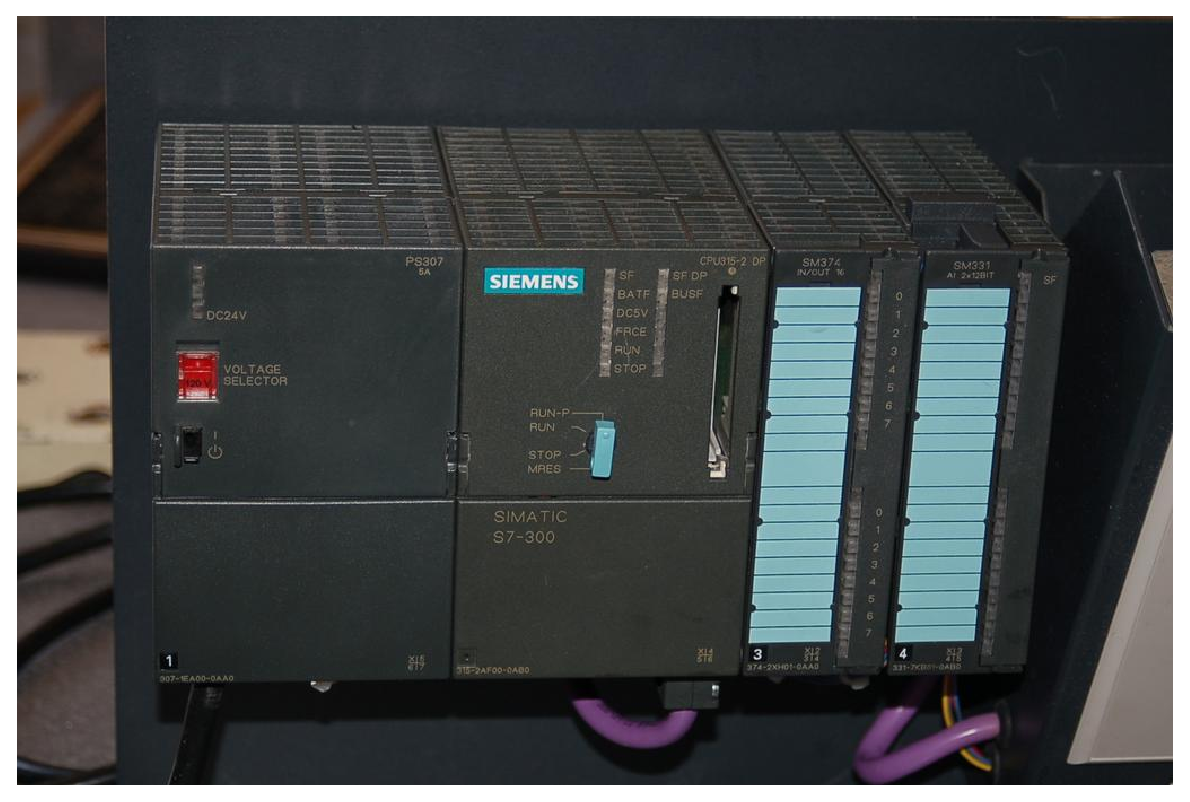
\includegraphics[width=0.7\textwidth]{plc_003.eps}$$
\end{frame}
\begin{frame}
	\frametitle{Eksempler på PLS-er}
$$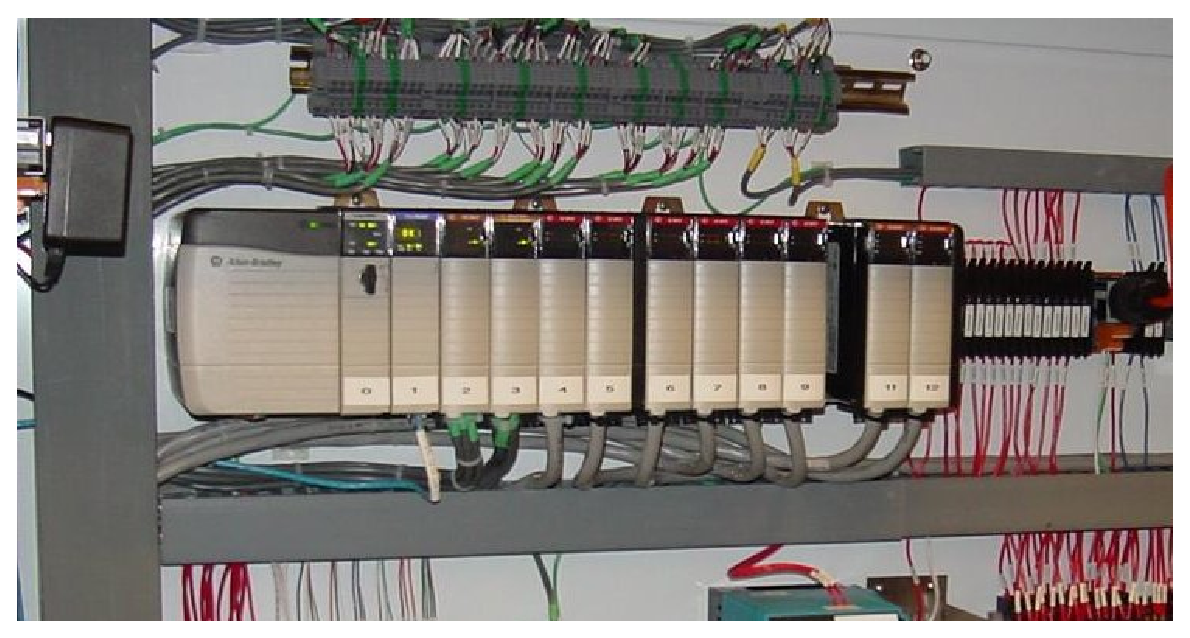
\includegraphics[width=0.9\textwidth]{plc_004.eps}$$
\end{frame}
\begin{frame}
	\frametitle{Eksempler på PLS-er}
$$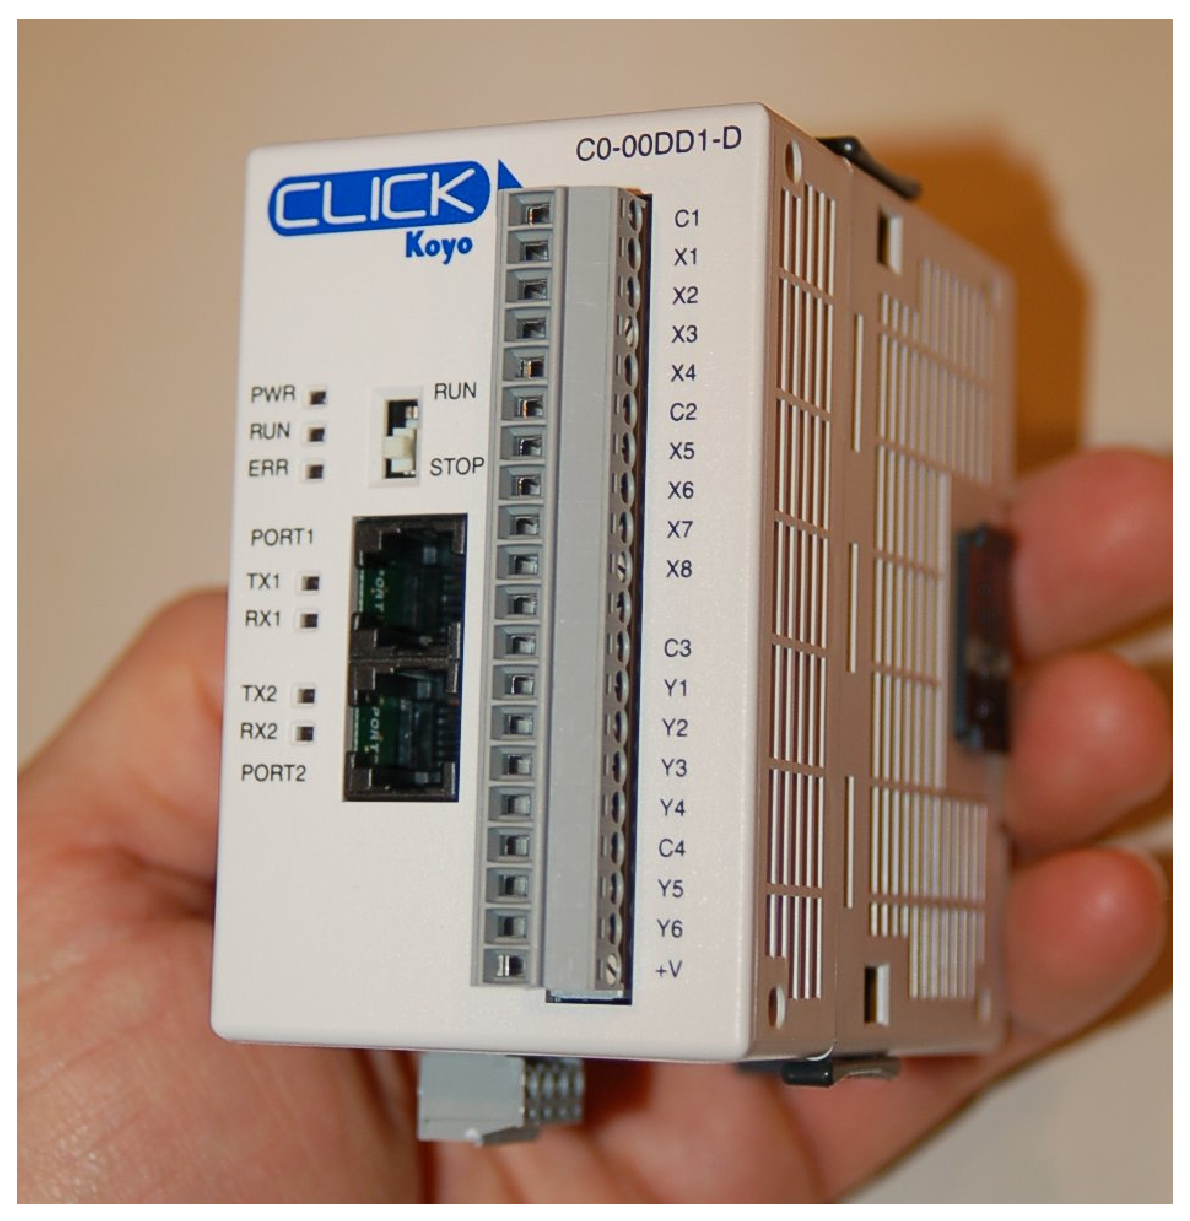
\includegraphics[width=0.5\textwidth]{plc_005.eps}$$
\end{frame}
\begin{frame}
	\frametitle{Eksempler på PLS-er}
$$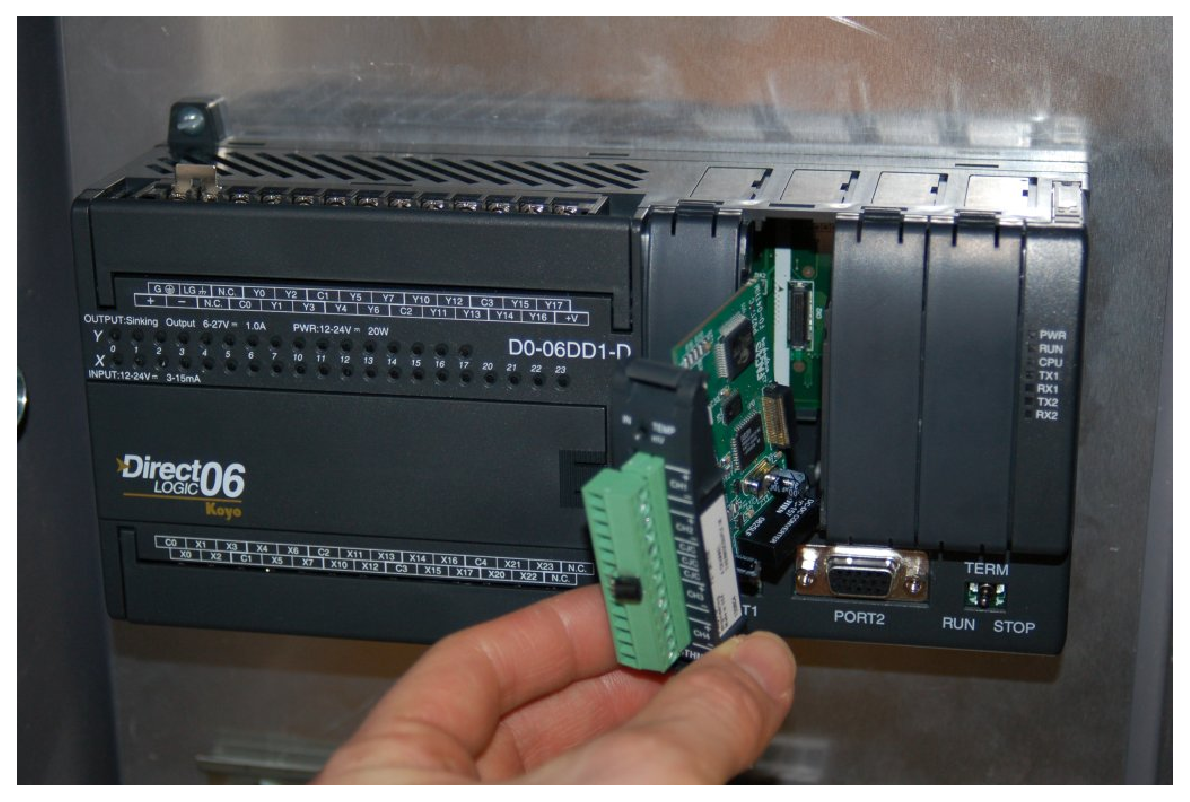
\includegraphics[width=0.8\textwidth]{plc_007.eps}$$
\end{frame}
\begin{frame}
	\frametitle{Eksempler på PLS-er}
$$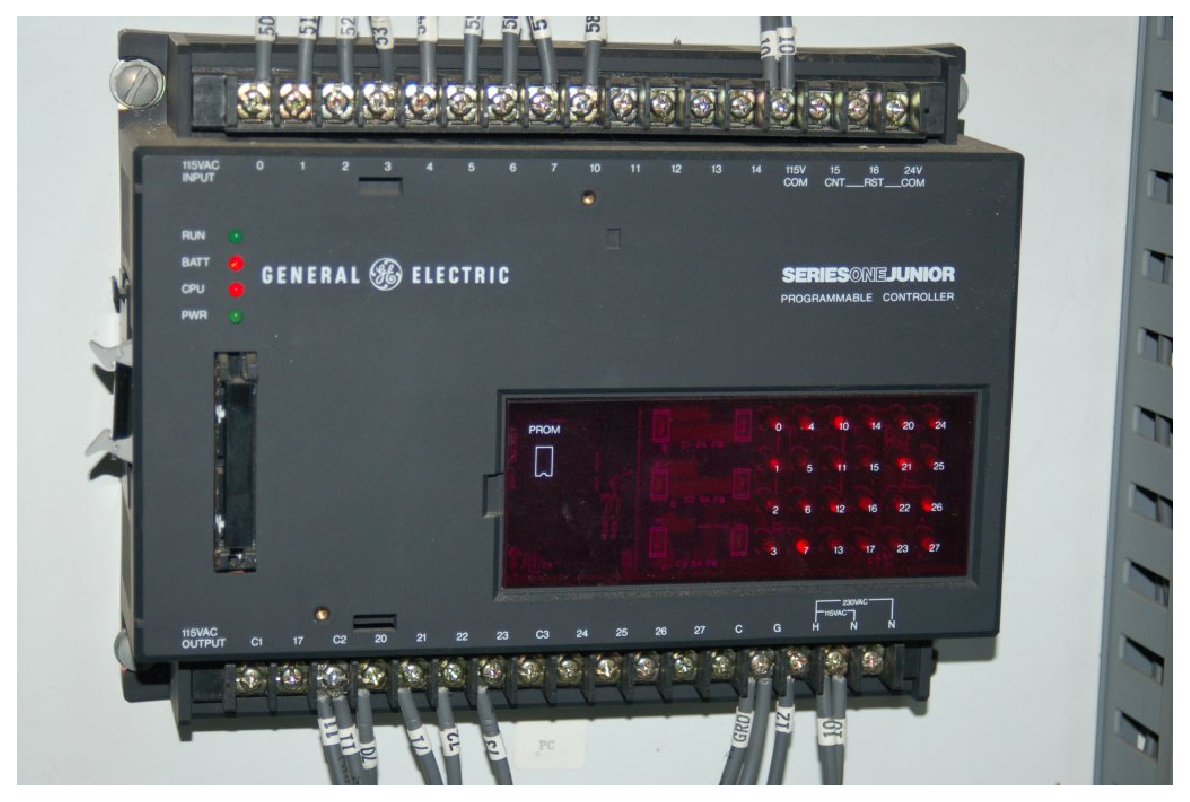
\includegraphics[width=0.8\textwidth]{plc_006.eps}$$
\end{frame}
\begin{frame}
	\frametitle{Inngangs- og utgangs tilkoblinger (IO-er)  }
	\framesubtitle{Tilgang til den virkelige verden}			
$$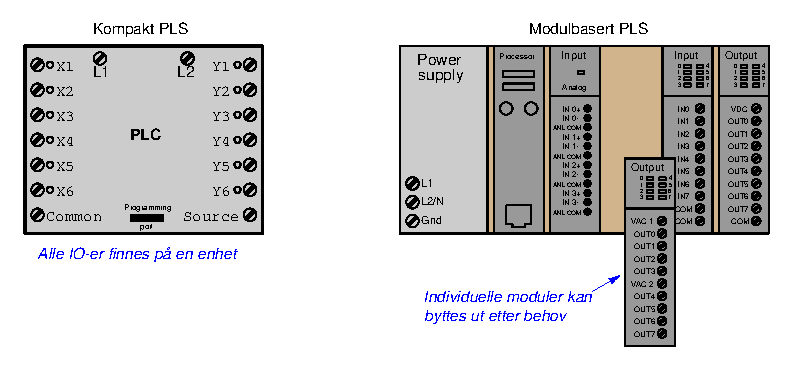
\includegraphics[width=0.8\textwidth]{plc_075.eps}$$
\end{frame}
\begin{frame}
	\frametitle{Inngangs- og utgangs tilkoblinger (IO-er)  }
	\framesubtitle{Tilgang til den virkelige verden}			
$$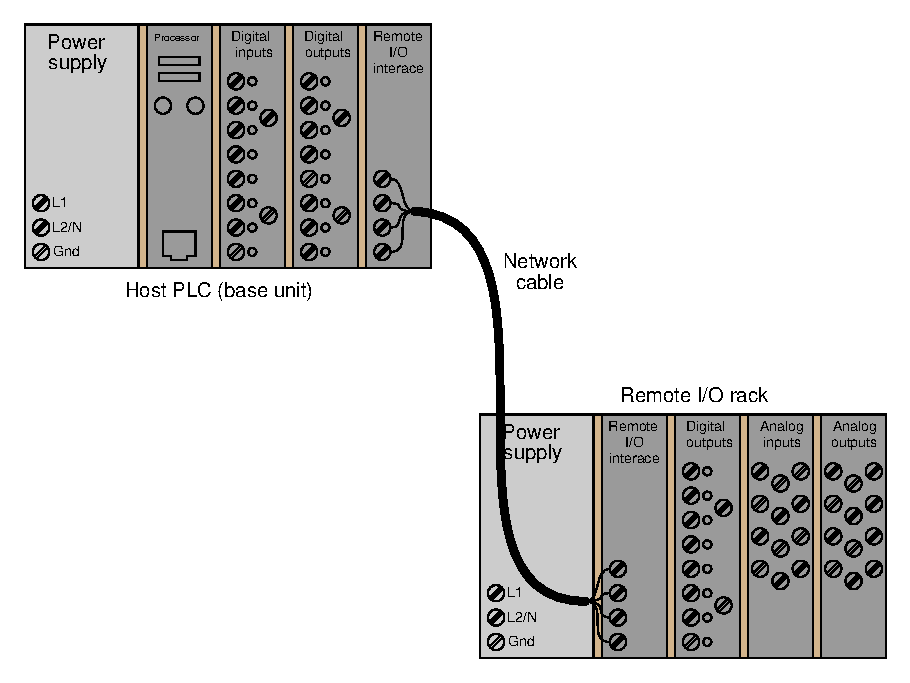
\includegraphics[width=0.6\textwidth]{plc_008.eps}$$
\end{frame}
\begin{frame}
	\frametitle{Galvaniske skiller}
	\begin{columns}
		\begin{column}{0.5\textwidth}
			\begin{itemize}
				\item \href{https://www.farnell.com/datasheets/73758.pdf}{\textbf{Isolerer}} PLS fra spenninger i felt. 
			\end{itemize}

			
		\end{column}

		\begin{column}{0.5\textwidth}
	$$\includegraphics[width=1\textwidth]{../output/noGPLimages/pls06.png}$$
		\end{column}
	\end{columns}
\end{frame}

\begin{frame}
	\frametitle{Digitale IO-er}
	\framesubtitle{Digital inngang}			
	Krav til PLS-IO er satt i \href{https://lese.standard.no/product/2503568/nb}{\textbf{NEK 61131-2}} --
	Eksempel på \href{https://www.ti.com/lit/ab/slla370d/slla370d.pdf}{\textbf{nyere inngang}}
$$\includegraphics[width=0.9\textwidth]{plc_073.eps}$$
\end{frame}

\begin{frame}
	\frametitle{Digitale IO-er}
	\framesubtitle{Digital utgang}			
$$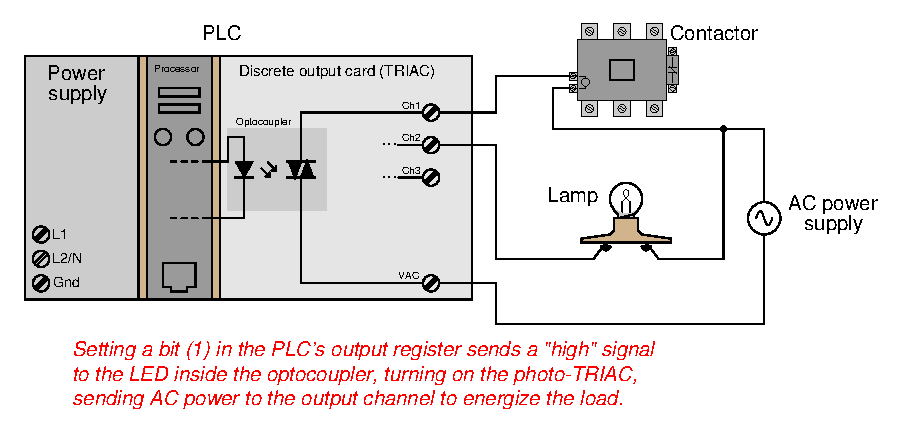
\includegraphics[width=0.9\textwidth]{plc_074.eps}$$
\end{frame}
\begin{frame}
	\frametitle{Sinking og Sourcing}
	\begin{columns}
		\begin{column}{0.5\textwidth}
		\begin{itemize}
			\item Inn- eller utgang som er sinking tar imot strøm 
			\item Inn- eller utgang som er soursing gir ut strøm 
		\end{itemize}	
		\end{column}
		\begin{column}{0.5\textwidth}

$$\includegraphics[width=0.9\textwidth]{plc_009.eps}$$
		\end{column}
	\end{columns}
\end{frame}


\begin{frame}
	\frametitle{Sinking og Sourcing}
	\begin{columns}
		\begin{column}{0.5\textwidth}
			
$$\includegraphics[width=0.9\textwidth]{plc_010.eps}$$
		\end{column}
		\begin{column}{0.5\textwidth}

$$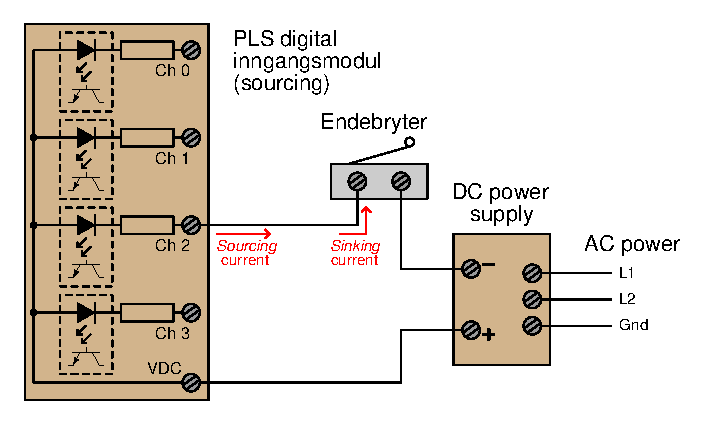
\includegraphics[width=0.9\textwidth]{plc_011.eps}$$
		\end{column}
	\end{columns}
\end{frame}
\begin{frame}
	\frametitle{Sinking og Sourcing}
	\begin{columns}
		\begin{column}{0.5\textwidth}
			
$$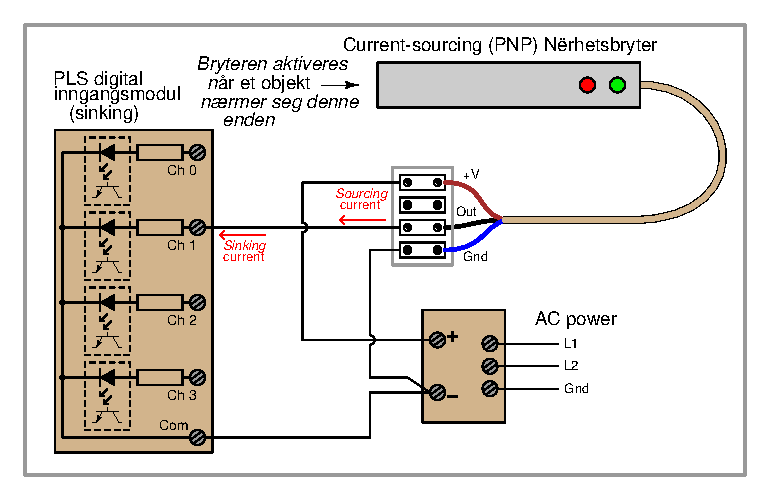
\includegraphics[width=1\textwidth]{plc_012_1.eps}$$
		\end{column}
		\begin{column}{0.5\textwidth}

$$\includegraphics[width=1\textwidth]{plc_012_2.eps}$$
		\end{column}
	\end{columns}
\end{frame}
\begin{frame}{Oppgave}
	\begin{columns}
		\begin{column}{0.3\textwidth}

			Hvilen er sinking og sourcring
			
		\end{column}

		\begin{column}{0.7\textwidth}
	$$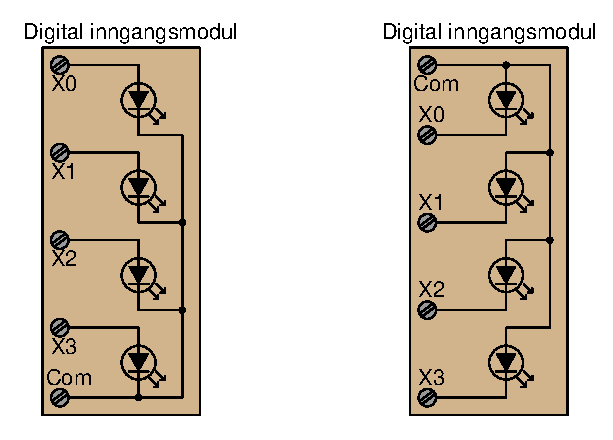
\includegraphics[height=0.8\textheight]{../src/i02359x01.eps}$$
		\end{column}
	\end{columns}
\end{frame}

\begin{frame}{Oppgave - 6ES7321-1BL00-0AA0}
	\begin{columns}
		\begin{column}{0.4\textwidth}

			Oppgaver: 
			\begin{itemize}
				\item Er dette en sinking eller sourcing PLS inngang 
				\item Tegn kobling for den øverste bryteren til inngang Ix0.4
				\item Tegn kobling for den nederste bryteren til inngang Ix0.7
			\end{itemize}
			
		\end{column}

		\begin{column}{0.6\textwidth}
			\href{https://docs.rs-online.com/4ccb/A700000009501908.pdf}{ 
			$$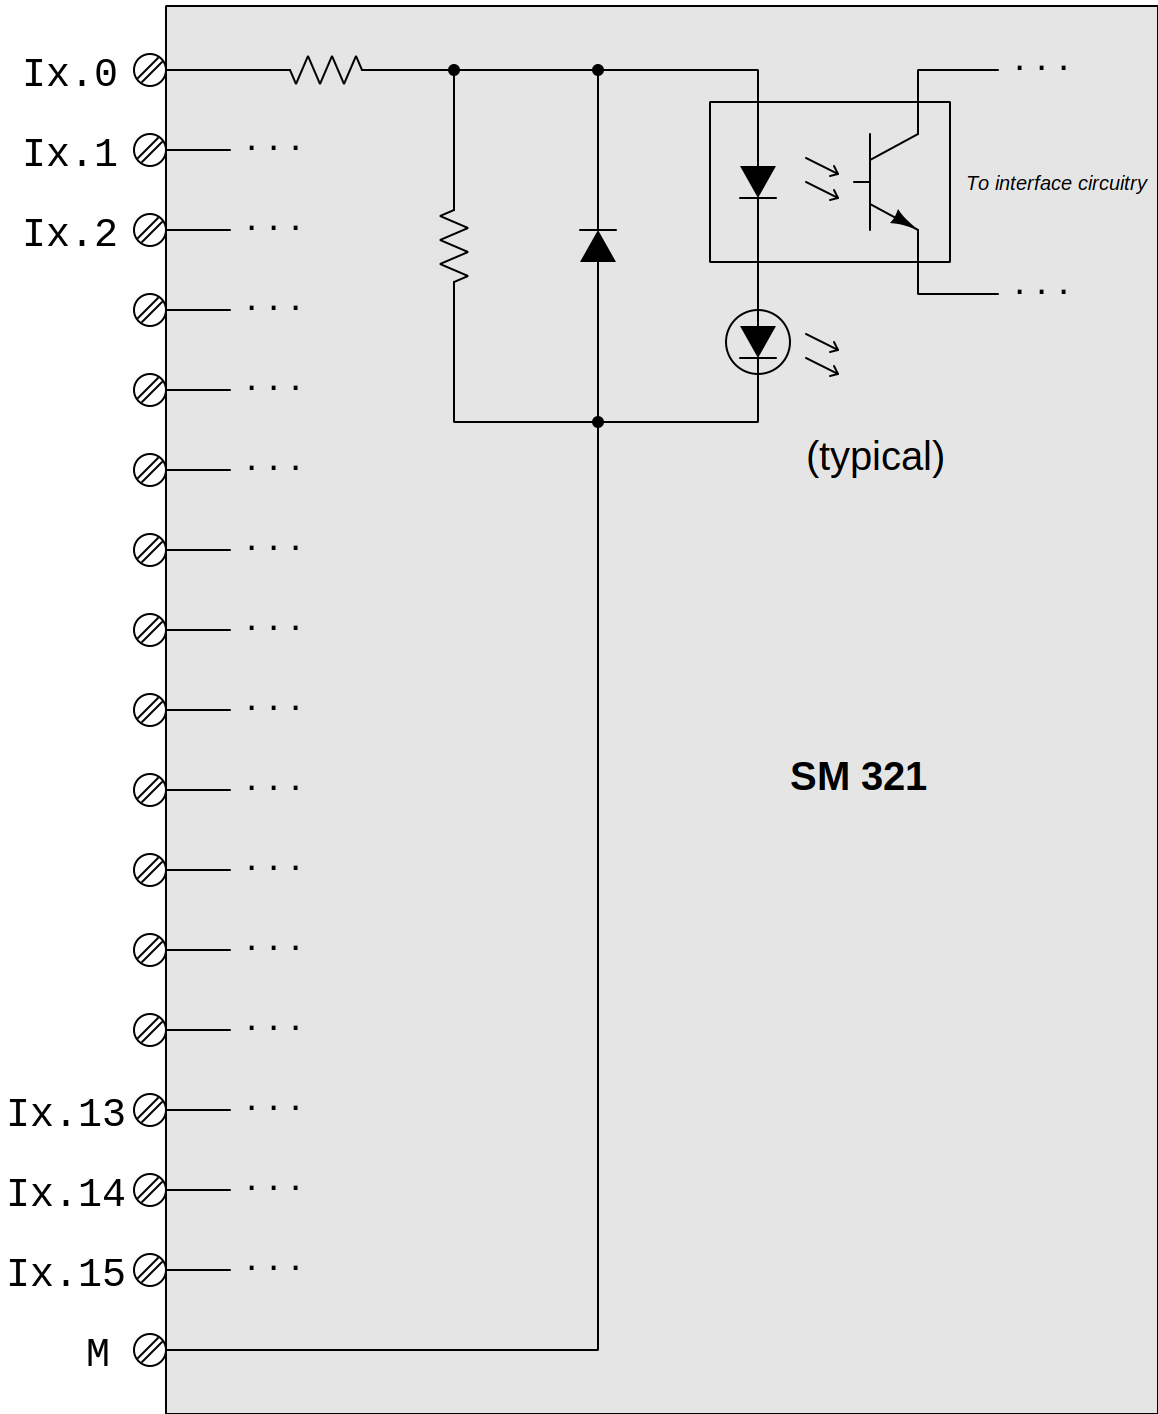
\includegraphics[height=0.8\textheight]{../src/i04536x01.eps}$$}
		\end{column}
	\end{columns}
\end{frame}
\begin{frame}{Oppgave}
	\begin{columns}
		\begin{column}{0.4\textwidth}

			Oppgaver: 
			\begin{itemize}
				\item Er dette en sinking eller sourcing PLS inngang 
				\item Tegn kobling for den øverste bryteren til inngang Ix0.4
				\item Tegn kobling for den nederste bryteren til inngang Ix0.7
			\end{itemize}
			
		\end{column}

		\begin{column}{0.6\textwidth}
	$$\includegraphics[height=0.8\textheight]{../src/i02508x01.eps}$$
		\end{column}
	\end{columns}
\end{frame}

\begin{frame}{Oppgave}
	\begin{columns}
		\begin{column}{0.4\textwidth}

			Oppgaver: 
			\begin{itemize}
				\item Hvilken koblings type har denne PLS-en
				\item Hvilken koblings type har denne sensoren
				\item Tegn kobling for den bryteren til inngang Ix0.5
			\end{itemize}
			
		\end{column}

		\begin{column}{0.6\textwidth}
	$$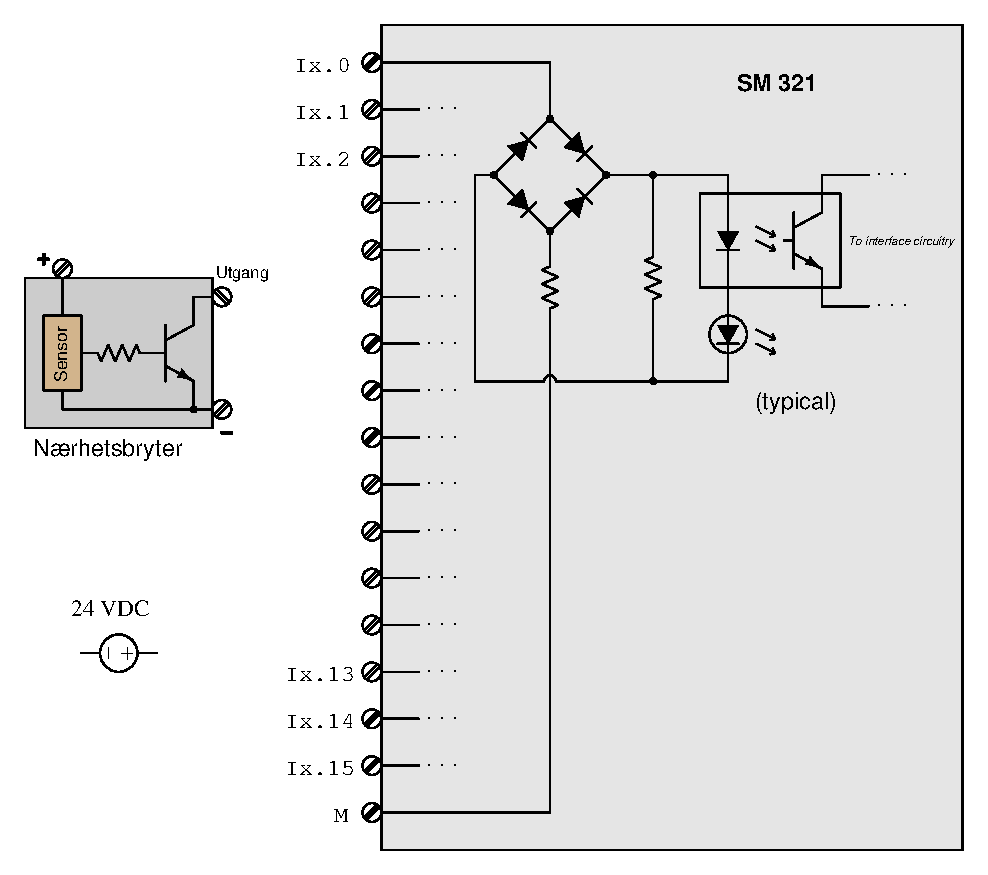
\includegraphics[height=0.8\textheight]{../src/i04544x01.eps}$$
		\end{column}
	\end{columns}
\end{frame}
\begin{frame}
	\frametitle{DO med rele}
	\begin{columns}
		\begin{column}{0.4\textwidth}
			Rele utganger :
			\begin{itemize}
				\item kan være potensialfrie
				\item Kan bryte forholdsvis store strømmer (6-10A)
				\item Kan brukes på AC og DC
			\end{itemize}

			
		\end{column}

		\begin{column}{0.6\textwidth}
	$$\includegraphics[height=0.6\textheight]{../output/noGPLimages/pls03.png}$$
		\end{column}
	\end{columns}
\end{frame}

\begin{frame}
	\frametitle{DO med transistor (Transistorutgang}
	\begin{columns}
		\begin{column}{0.5\textwidth}
			Transistorutganger:
			\begin{itemize}
				\item bryter mindre strømmer (0.5 og 1 A er vanlig)
				\item bryter raskere en rele utganger
				\item Finnes i NPN eller PNP utgaver
				\item NPN kalles også low side switching
				\item PNP kalles også high side switching
				\item Kan brukes på DC
			\end{itemize}

			
		\end{column}

		\begin{column}{0.5\textwidth}
	$$\includegraphics[width=1\textwidth]{../output/noGPLimages/pls04.png}$$
		\end{column}
	\end{columns}
\end{frame}

\begin{frame}
	\frametitle{DO med triac}
	\begin{columns}
		\begin{column}{0.5\textwidth}
			\begin{itemize}
				\item Kan bryte mindre AC strømmer en releer
				\item Tåler flere bryte sykluser
			\end{itemize}

			
		\end{column}

		\begin{column}{0.5\textwidth}
	$$\includegraphics[width=0.8\textwidth]{../output/noGPLimages/pls05.png}$$
		\end{column}
	\end{columns}
\end{frame}

\begin{frame}{Oppgave}
	\begin{columns}
		\begin{column}{0.4\textwidth}

			Oppgaver: 
			\begin{itemize}
				\item Hvilken oppgave har dioden på releet?
				\item Hvilken oppgave har dioden parallellt med utgangstransistoren?
				\item Hvilken oppgave har dioden i serie med optokobleren?
				\item Er det en sinking eller sourcsing PLS utgang?
				\item Tegn kobling som er nødvendig for å få releet til å virke 
			\end{itemize}
			
		\end{column}

		\begin{column}{0.6\textwidth}
	$$\includegraphics[height=0.8\textheight]{../src/i04537x01.eps}$$
		\end{column}
	\end{columns}
\end{frame}

\begin{frame}{Oppgave}
	\begin{columns}
		\begin{column}{0.4\textwidth}

			Oppgaver: 
			\begin{itemize}
				\item Tegn kobling for releet til Qx.5 
				\item Tegn kobling for solonoiden til Qx.7
			\end{itemize}
			
		\end{column}

		\begin{column}{0.6\textwidth}
	$$\includegraphics[height=0.8\textheight]{../src/i04246x01.eps}$$
		\end{column}
	\end{columns}
\end{frame}

\begin{frame}{Oppgave}
	Du skal koble opp PLS-en på neste slide. Koble til PSH som sinking sensor og PSL som sourcing sensor. Releene er 220V 
\end{frame}
\begin{frame}{Oppgave}
	$$\includegraphics[height=0.5\textheight]{../src/i02379x01.eps}$$
\end{frame}


\begin{frame}{Oppgave}
	Du skal koble opp PLS-en på neste slide. SSR-ene skal ha 24V
\end{frame}
\begin{frame}{Oppgave}
	$$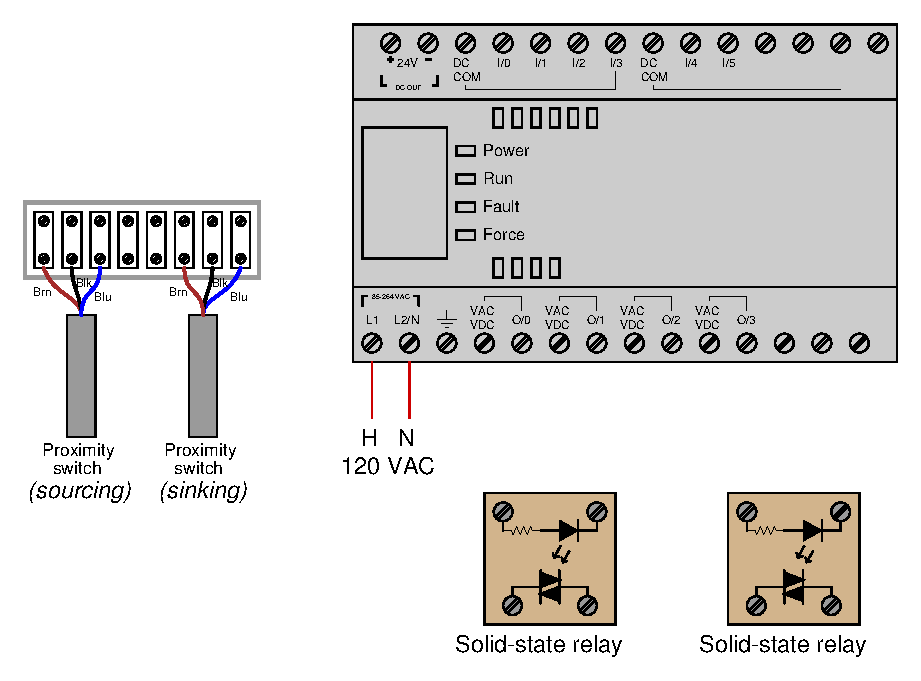
\includegraphics[height=0.7\textheight]{../src/i04524x01.eps}$$
\end{frame}
\begin{frame}{Oppgave}

			Anta at du har fått i oppdrag å koble disse tre trykkbrterene til DI-ene IN-4, IN-6 og IN-13 på en Allen-Bradley model 1756-IA16. Se neste slide. 
			
Tegn inn de nødvendige koblingene for at trykkbryterene skal virke på de spesifiserte DI-ene. Ta med eventuelt nødvendige spenningskilder. 
	Tips: Det kan hjelpe deg om du søker opp et dokument som kalles \href{https://literature.rockwellautomation.com/idc/groups/literature/documents/td/1756-td002_-en-e.pdf}{ \textbf{``1756 ControlLogix I/O Modules''}(publication 1756-TD002A-EN-E, May 2009)}
\end{frame}
\begin{frame}{Oppgave}
$$\includegraphics[width=10cm]{../src/i02060x01.eps}$$
\end{frame}

\section{Analog instrumentering}


\begin{frame}
	\frametitle{Analog instrumentering}
	\begin{columns}
		\begin{column}{0.5\textwidth}
			Et analogt singal er en spenning eller en strøm som er proporsjonal med en fysisk måling.
Betegnelsen analog henspeiler på egenskapen til hva som måles og ikke hvordan signalet
behandles internt i PLS eller måleutstyr (her behandles det ofte digitalt).
		\end{column}
		\begin{column}{0.5\textwidth}
		\end{column}
	\end{columns}
\end{frame}
\begin{frame}
	\frametitle{4 til 20 mA analoge strøm signaler }
	\begin{columns}
		\begin{column}{0.5\textwidth} 
			Den mest vanlige måten å overføre analoge signaler i automatiserteanlegg er med en 4-20 mA strømsløyfe. Dette er en \textit{analog}signal standard. Det betyr at verdien på  trømmen angir et signal fra 0-100\%(4-20 mA)

		\end{column}
		\begin{column}{0.5\textwidth}
			\begin{tabular}{|l|c|r|}
			\noalign{\hrule}
			\textbf{Current value} & \textbf{\% of scale} \cr
			\noalign{\hrule}
			4 mA & 0\% \cr
			\noalign{\hrule}
			% Another row
			8 mA & 25\% \cr
			\noalign{\hrule}
			12 mA & 50\% \cr
			\noalign{\hrule}
			16 mA & 75\% \cr
			\noalign{\hrule}
			20 mA & 100\% \cr
			\noalign{\hrule}
			\end{tabular}
		\end{column}
	\end{columns}
\end{frame}

\begin{frame}
	\frametitle{4 til 20 mA analoge strøm signaler }
	\begin{columns}
		\begin{column}{0.5\textwidth} 
			Om vi for eksempel setter opp en temperaturtransmitter til å måle et temperaturområde på 50-250°C, vil temperaturen i forhold til strøm gi følgende graf. 
		\end{column}
		\begin{column}{0.5\textwidth}
			$$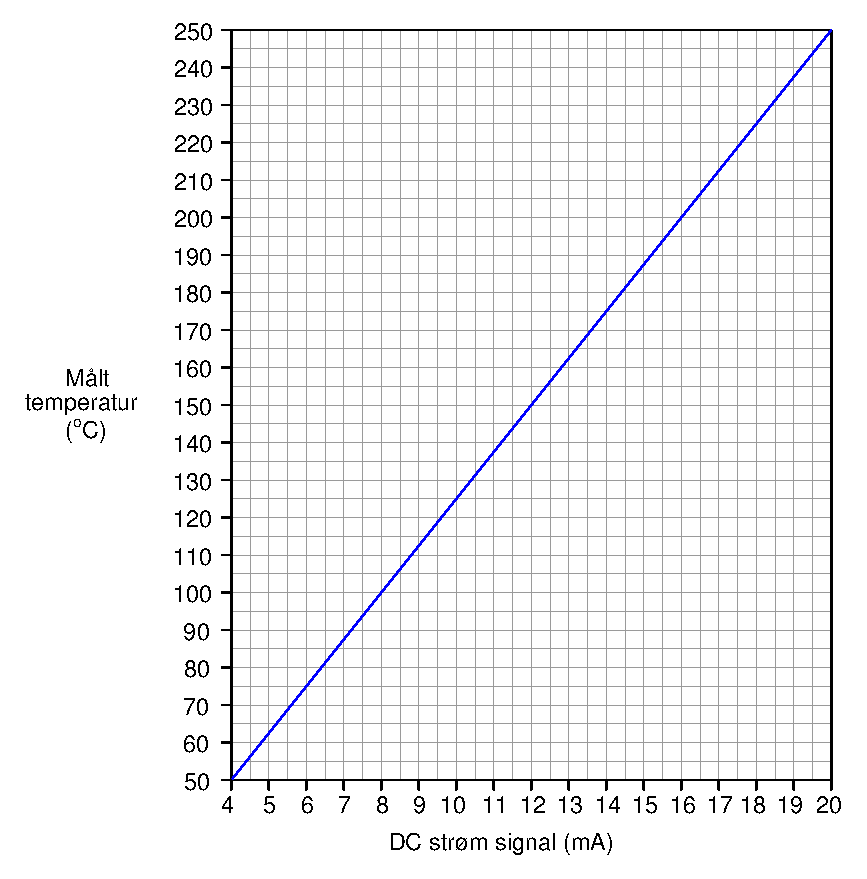
\includegraphics[height=0.8\textheight]{current01.eps}$$
		\end{column}
	\end{columns}
\end{frame}


\begin{frame}
	\frametitle{Tilpassede overføringsenheter}
	\begin{columns}
		\begin{column}{0.4\textwidth} 
Et viktig konsept i analog instrumentering er at enheter som sender og mottar må være tilpasset i måleområde til hveradre. 
\vskip 0.1 cm
Legg merke til hvordan utgangsområdet for hver enhet passer med inngangsenheten som skal motta signalet. I målesystemet må kommunikasjonen mellom hver mottaker og sender være avklart på forhånd, om den ikke er det vil ikke avlesningen av signalet ha noen sammenheng med det målte signalet. 
		\end{column}
		\begin{column}{0.6\textwidth}
			$$\includegraphics[height=0.6\textheight]{current60.eps}$$
		\end{column}
	\end{columns}
\end{frame}
\begin{frame}
	\frametitle{Sammenhengen mellom 4-20mA signal og andre signaler}
	\begin{columns}
		\begin{column}{0.5\textwidth} 
Et 4-20mA strømsignal representerer et eller annet signal fra 0-100\%. Denne sammenhengen er vanligvis lineær. 
\vskip 0.2cm
Siden dette er en lineær funksjon, kan vi bruke formelen for en rett linje til å relatere rett signal \% til strømverdier.
\vskip 0.2cm
$$y = mx + b$$
$y$ = Utgangen fra instrumentet

$x$ = Inngangen fra instrumentet

$m$ = Stigningstallet for linjen

$b$ = $y$-skjeringspunktet (m.a.o. \textit{aktivt} nullpunkt for instrumentutgangen. \index{aktivt nullpunkt}) Denne vil vi kalle $y_{start}$ fra nå av. 
		\end{column}
		\begin{column}{0.5\textwidth}
			$$\includegraphics[height=0.7\textheight]{current42.eps}$$
		\end{column}
	\end{columns}
\end{frame}
%\section{Sammenhengen mellom 4-20mA signal og andre signaler}
%
%
%
%$$\includegraphics{current42.eps}$$
%
%\label{instrument_range_linear_equation}
%
%
%
%
%\noindent
%Hvor,
%
%\vskip 10pt
%
%Med en gang vi har passende verdier for $m$ og $y_{start}$, kan vi bruke formelen for en rett linje for å konvertere mellom inn og utgangen på en transmitter. 
%
%Før vi kan bruke formelen må vi finne verdiene for stigningstallet og y-skjæringspunktet for den transmitteren vi jobber med.  
%
%For den lineære funksjonen som vises skal vi finne stigningstallet ($m$) ved å dele linjens $y_{range}$ med linjens $x_{range}$. $y_{range}$ er transmitterens inngangsområde, og $x_{range}$ er transmitteres utgangsområde. 
%
\begin{frame}
	\frametitle{Konvertering mellom inn- og utgang}
	\begin{columns}
		\begin{column}{0.5\textwidth} 
$$m =\dfrac{ y_{range}} {x_{range}} = \dfrac {20 - 4} {100 - 0} = \dfrac{ 16} {100}$$
$$y = \dfrac{ y_{range}} {x_{range}}x + b$$
Om vi tar hensyn til at heller ikke x-aksen starter på null kan vi sette opp denne formelen: 
$$\dfrac{y-y_{start}}{y_{range}}=\dfrac{x-x_{start}}{x_{range}}$$
		\end{column}
		\begin{column}{0.5\textwidth}
			$$\includegraphics[height=0.8\textheight]{current43.eps}$$
		\end{column}
	\end{columns}
\end{frame}

\begin{frame}
	\frametitle{Konvertering mellom inn- og utgang}
	\begin{columns}
		\begin{column}{0.5\textwidth} 
Vi kan nå bruke denne formelen for å regne ut hvor mange milliamper en gitt prosent inngangssignal tilsvarer. Vi kan f.eks. bruke et inngangsignal på 34.7\% til å regne ut tilhørende milliamper verdi:
\vskip 0.5cm
\begin{align*}
	y &= \left({16 \over 100}\right)34.7 + 4\\
	y &= 5.552 + 4\\
	y &= 9.552
\end{align*}
		\end{column}
		\begin{column}{0.5\textwidth}
			$$\includegraphics[height=0.4\textheight]{current63.eps}$$
		\end{column}
	\end{columns}
\end{frame}

\begin{frame}
	\frametitle{Formelen med transmitter begreper}
			$$\includegraphics[height=0.5\textheight]{current59.eps}$$
\end{frame}
\begin{frame}
	\frametitle{Oppgave: Regulatorutgang til reguleringsventil.}
	\begin{columns}
		\begin{column}{0.5\textwidth} 
\textit{En PID regulator sender et utgangsignal til en direkteverkende reguleringsventil (d.v.s 4mA er lukket og 20mA er helt åpen).Hvor åpen (0-100\%i) vil reguleringsventilen være med dette signalet?}
		\end{column}
		\begin{column}{0.5\textwidth}
			$$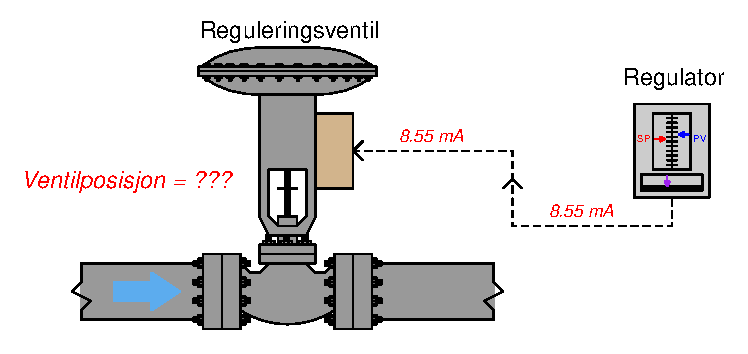
\includegraphics[height=0.35\textheight]{current44.eps}$$
		\end{column}
	\end{columns}
\end{frame}
\begin{frame}
	\frametitle{Oppgave: Regulatorutgang til reguleringsventil.}
	\begin{columns}
		\begin{column}{0.5\textwidth} 
\textit{En PID regulator sender et utgangsignal til en direkteverkende reguleringsventil (d.v.s 4mA er lukket og 20mA er helt åpen).Hvor åpen (0-100\%i) vil reguleringsventilen være med dette signalet?}
	\begin{align*}
		\dfrac{y-y_{start}}{y_{range}}&=\dfrac{x-x_{start}}{x_{range}}\\
		\dfrac{8.55-4}{16}&=\dfrac{x-0}{100}\\
		\dfrac{100 \cdot 4.55}{16}&=x\\
		x&={28.4}\\
	\end{align*}
		\end{column}
		\begin{column}{0.5\textwidth}
			$$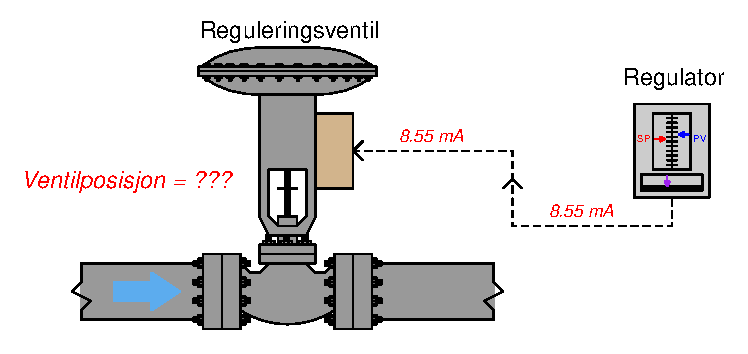
\includegraphics[height=0.35\textheight]{current44.eps}$$
		\end{column}
	\end{columns}
\end{frame}

\begin{frame}
	\frametitle{Oppgave: Strømningsmåler}
	\begin{columns}
		\begin{column}{0.5\textwidth} 
\textit{En strømningsmåler har et måleområde på 0 til 1400 liter per minutt. Regn ut strømsignalet med en strømningsrate på 816 l/m.}
\vskip 4cm
.
		\end{column}
		\begin{column}{0.5\textwidth}
			$$\includegraphics[height=0.3\textheight]{current45.eps}$$
		\end{column}
	\end{columns}
\end{frame}
\begin{frame}
	\frametitle{Oppgave: Strømningsmåler}
	\begin{columns}
		\begin{column}{0.5\textwidth} 
\textit{En strømningsmåler har et måleområde på 0 til 1400 liter per minutt. Regn ut strømsignalet med en strømningsrate på 816 l/m.}
	\begin{align*}
		\dfrac{y-y_{start}}{y_{range}}&=\dfrac{x-x_{start}}{x_{range}}\\
		\dfrac{y-4}{16}&=\dfrac{816-0}{1400}\\
		y&=\dfrac{816\cdot16}{1400}+4\\
		y&={13.3mA}\\
	\end{align*}

		\end{column}
		\begin{column}{0.5\textwidth}
			$$\includegraphics[height=0.3\textheight]{current45.eps}$$
		\end{column}
	\end{columns}
\end{frame}
\begin{frame}
	\frametitle{PLS med analog inngang}
	\begin{columns}
		\begin{column}{0.5\textwidth} 
			\textit{En Allen-Bradley SLC500 PLS bruker en 16-bit analog-til-digital omformer i AI kortet 1746-NI4. I dette kortet konverteres 4-20 mA til digitale nummer(integere) fra 3277 (ved 4 mA) til 16384 (ved 20 mA). I en PLS-en skal denne verdien vises på et display (HMI). En verdi fra 3277-16384 vil ikke være særlig nyttig for en operatør. Derfor må disse verdiene skalleres ved å regne de om til 0-700 l/m.} 
		\end{column}
		\begin{column}{0.5\textwidth}
			$$\includegraphics[height=0.6\textheight]{current53.eps}$$
		\end{column}
	\end{columns}
\end{frame}
\begin{frame}
	\frametitle{PLS med analog inngang}
	\begin{columns}
		\begin{column}{0.5\textwidth} 
			\textit{En verdi fra 3277-16384 vil ikke være særlig nyttig for en operatør. Derfor må disse verdiene skalleres ved å regne de om til 0-700 l/m.} 
			\vskip 4cm .
		\end{column}
		\begin{column}{0.5\textwidth}
		\end{column}
	\end{columns}
\end{frame}
\begin{frame}
	\frametitle{4-leder strømsløyfe med ekstern strømforsyning }
			$$\includegraphics[height=0.8\textheight]{current09.eps}$$
\end{frame}
\begin{frame}
	\frametitle{4-leder strømsløyfe med internstrømforsyning}
			$$\includegraphics[height=0.8\textheight]{current10.eps}$$
\end{frame}
\begin{frame}
	\frametitle{2-leder strømsløyfe med intern strømforsyning}
			$$\includegraphics[height=0.8\textheight]{current11.eps}$$
\end{frame}
\begin{frame}
	\frametitle{4-leder strømsløyfe passiv eller aktiv transmitter}
			$$\includegraphics[height=0.8\textheight]{current61.eps}$$
\end{frame}
\begin{frame}
	\frametitle{Bruk av vanlig ampermeter til målinger i strømsløyfer}
			$$\includegraphics[height=0.8\textheight]{current05.eps}$$
\end{frame}
\begin{frame}
	\frametitle{Bruk av vanlig ampermeter til målinger i strømsløyfer}
			$$\includegraphics[height=0.8\textheight]{current26.eps}$$
\end{frame}

\begin{frame}
	\frametitle{Oppgave}

	\footnotesize

$$\includegraphics[width=9cm]{../src/i02273x01.eps}$$

Vis hvordan feltutstyret skal kobles til regulatoren, inkluder plassering av motstander for konvertere strømsignal til spenningssignal som regulatorens ADC kan lese. Bruk skjermet kabel og vis hvordan denne skal jordes. 
\normalsize
\end{frame}

\begin{frame}
	\frametitle{Alternativ}
			$$\includegraphics[height=0.8\textheight]{current27.eps}$$
\end{frame}
\begin{frame}
	\frametitle{Alternativ}
			$$\includegraphics[height=0.4\textheight]{current06.eps}$$
\end{frame}
\begin{frame}
	\frametitle{Alternativ}
			$$\includegraphics[height=0.7\textheight]{current07.eps}$$
\end{frame}
\begin{frame}
	\frametitle{Alternativ}
			$$\includegraphics[height=0.7\textheight]{current28.eps}$$
\end{frame}

\section{Analog til Digital omforming ADC}
\begin{frame}
	\frametitle{Analog til Digital omforming ADC}
	\begin{columns}

		\begin{column}{0.5\textwidth} 
			For at PLS programet skal kunne behandle et analogt signal må det digitaliseres. Dette gjøres i en Analog to Digital Converter eller ADC. 
		\end{column}
		\begin{column}{0.5\textwidth}
			$$\includegraphics[height=0.5\textheight]{ADC.pdf}$$
		\end{column}
	\end{columns}
\end{frame}
\begin{frame}
	\frametitle{ADC oppløsning}
	\begin{columns}

		\begin{column}{0.5\textwidth} 
Dette er en 12-bit ADC. Om spenningen inn på omformern er 1-5V, er den analoge rangen 4V. Vi kan da dele opp denne rangen i $2^{12}-1$ ulike steg. Den analoge oppløsningen blir da. 

			$$\text{Analog oppløsning} = \dfrac{\text{Analog span}}{2^n - 1}=\dfrac{4V}{2^{12}-1}=0.98mV$$

		\end{column}
		\begin{column}{0.5\textwidth}
			$$\includegraphics[height=0.4\textheight]{digital_01.eps}$$
		\end{column}
	\end{columns}
\end{frame}

\begin{frame}
	\frametitle{ADC samplingsintervall og aliasing (sampling rate)}
	\begin{columns}
		\begin{column}{0.5\textwidth} 
			Om vi ikke sampler minst to ganger pr. periode kan vi få et fenomen som kalles aliasing. Det vil si at ADC-en gjengir en annen frekvens en den som ble sendt inn. Det er en god regel å sample med en hastighet som er 10 ganger den høyeste frekvensen som en er interesert i. 
		\end{column}
		\begin{column}{0.5\textwidth}
			$$\includegraphics[width=1\textwidth]{digital_02.eps}$$
			$$\includegraphics[width=1\textwidth]{digital_79.eps}$$
		\end{column}
	\end{columns}
\end{frame}
\begin{frame}
	\frametitle{Anti-aliasing filter}
	\begin{columns}
		\begin{column}{0.5\textwidth} 
			Ved å sette inn et filter som tar vekk høye frevenser kan en unngå problemene med aliasing. Det er vanlig å kalle dette for anti-aliasing filter
		\end{column}
		\begin{column}{0.5\textwidth}
			$$\includegraphics[width=1\textwidth]{digital_03.eps}$$
		\end{column}
	\end{columns}
\end{frame}


\end{document}
